\documentclass{standalone}

\usepackage{tikz}

\newcommand{\vb}{\mathbf}

\begin{document}

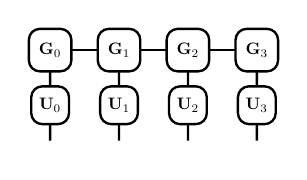
\begin{tikzpicture}[scale=0.7, every node/.style={scale=0.6}]

    \node[draw, rounded corners, minimum size=0.9cm, inner sep=0.5, line width=0.3mm] (G1) at (9.0+1.25,0.5) {$\vb{G}_{0}$};
    \node[draw, rounded corners, minimum size=0.9cm, inner sep=0.5, line width=0.3mm] (G2) at (10.25+1.25,0.5) {$\vb{G}_{1}$};
    \node[draw, rounded corners, minimum size=0.9cm, inner sep=0.5, line width=0.3mm] (G3) at (11.5+1.25,0.5) {$\vb{G}_{2}$};
    \node[draw, rounded corners, minimum size=0.9cm, inner sep=0.5, line width=0.3mm] (G4) at (12.75+1.25,0.5) {$\vb{G}_{3}$};

    \draw[line width=0.3mm] (G1) -- (G2) -- (G3) -- (G4);

    \node[draw, rounded corners, minimum size=0.8cm, inner sep=0.0, line width=0.3mm] (Q1b) at (9.0+1.25,-0.5) {$\vb{U}_{0}$};
    \node[draw, rounded corners, minimum size=0.8cm, inner sep=0.0, line width=0.3mm] (Q2b) at (10.25+1.25,-0.5) {$\vb{U}_{1}$};
    \node[draw, rounded corners, minimum size=0.8cm, inner sep=0.0, line width=0.3mm] (Q3b) at (11.5+1.25,-0.5) {$\vb{U}_{2}$};
    \node[draw, rounded corners, minimum size=0.8cm, inner sep=0.0, line width=0.3mm] (Q4b) at (12.75+1.25,-0.5) {$\vb{U}_{3}$};

    \draw[line width=0.3mm] (G1) -- (Q1b);
    \draw[line width=0.3mm] (G2) -- (Q2b);
    \draw[line width=0.3mm] (G3) -- (Q3b);
    \draw[line width=0.3mm] (G4) -- (Q4b);

    \node (Q1c) at (9.0+1.25,-1.25) {};
    \node (Q2c) at (10.25+1.25,-1.25) {};
    \node (Q3c) at (11.5+1.25,-1.25) {};
    \node (Q4c) at (12.75+1.25,-1.25) {};

    \draw[line width=0.3mm] (Q1b) -- (Q1c);
    \draw[line width=0.3mm] (Q2b) -- (Q2c);
    \draw[line width=0.3mm] (Q3b) -- (Q3c);
    \draw[line width=0.3mm] (Q4b) -- (Q4c);
\end{tikzpicture}

\end{document}
